\documentclass[a4paper,12pt]{article}
\usepackage[a4paper,inner=1cm, outer=1.5cm, top=1cm, bottom=2cm,bindingoffset =.9cm]{geometry}

\usepackage[english]{babel}
\usepackage{blindtext}
\usepackage{microtype}
\usepackage{graphicx}
\usepackage{wrapfig}
\usepackage{enumitem}
\usepackage{fancyhdr}
\usepackage{amsmath,amssymb,amsthm}
\usepackage{index}




\title{\Large{\textbf {PROFESSOR -COURSE OPTIMISATION: A CASE STUDY OF IMPLEMENTATION OF GRAPH THEORY}}}
\author{By  Ayananshu Mohanty, T Saket Hatwar, Yash Chaphekar}
\date{17 November 2023}


\begin{document}

\small
\pagenumbering {arabic}
\setcounter{page}{1}
\fancyhf{}
\renewcommand{\headrulewidth}{2pt}
\renewcommand{\footrulewidth}{1pt}

\maketitle


\textbf{\textbf{
\\ \\ Abstract –This paper analyses the problem of assigning different courses to professors in a single semester. To achieve the desired output, graph optimization was implemented. The paper goes into detail explaining the problem statement, the methods developed to tackle the problem, and specific test cases to check how the code written functions. We also look into the limitations of our solution and discuss if any better methods are possible to implement.
}}

\section{Introduction}
(i)\textbf{ Professor-Course Optimization} refers to assigning each course available in a semester to a professor according to his/her preferences. Each professor can take either 1 full course, share 1 course with another professor, or take 1 full course and share the other in the same semester. Thus, a professor can take either 0.5, 1, or 1.5 courses in a semester. The courses can be classified into 4 types.\textbf{ First Degree CDC, Higher Degree CDC, First Degree Elective, Higher Degree Elective. }It is mandatory to make sure that each CDC is assigned to a professor. The electives are assigned in such a way that the maximum number of electives can be offered in a semester. \\ \\
(ii)Each professor will give a list in which they give their priorities for each course of every type. Every professor must give at least 4 First Degree CDCs, 4 Higher Degree CDCs, 2 First Degree Electives, and 2 Higher Degree electives as their course preferences. The task on hand is to make sure that each professor is assigned the courses that are at the top of their priority orders and make an optimized solution for the professor to course mapping. \\ \\
(iii) The two methods proposed to solve the problem were the Genetic Algorithm approach and the Graph algorithm approach. 
\section {Proposed approach}
(i)\textbf{Genetic algorithm
\footnote{ The genetic algorithm serves as an approach for tackling optimization problems, whether constrained or unconstrained, drawing inspiration from the mechanism of natural selection observed in biological evolution. It iteratively adjusts a population of individual solutions to refine and improve their effectiveness in solving the given problem.}:}

 The procedure followed in the genetic algorithm approach is as follows-\\ \\
a)\textbf{Initialization:} A population of potential solutions is randomly generated. Each solution represents one solution to the optimization problem. In the context of our problem, this refers to assigning professors to their courses of highest priority without taking into consideration how many professors are assigned to one course.\\ \\
b)\textbf{Selection:} Some individuals from the current population are selected to form the new generation. The selection is based on the “fitness” \footnote{Refers to a score which is calculated to optimize based on certain parameters.} of each individual, and the individuals with higher fitness levels have a higher chance of getting selected. In the context of our problem, this fitness score is calculated by assigning numbers and priorities to each type of course available, i.e.) First Degree CDC gets a score of 1, Higher Degree CDC gets a score of 2, etc. Based on the preferences that the professor has filled, the fitness score is calculated with respect to the course assigned to them. The lower the score is, the better the course assignment becomes to the professor.\\ \\
c)\textbf{Recombination}: Pairs of individuals are chosen to mate, and a crossover operation is applied to their genetic representations. \\ \\
d)\textbf{Mutation}: Random changes are applied to certain individuals in the population. This introduces genetic diversity and helps explore the solution space in a better way \\ \\
e)\textbf{Evaluation}: The fitness of each individual in the new population is evaluated. The fitness function measures how well a solution solves the optimization problem. \\ \\
f)\textbf{Termination}: The algorithm keeps repeating until a termination condition is met (e.g., a satisfactory solution is found. After each iteration, the courses assigned to the professors get more and more optimized. This means that each professor gets their top priority courses.
 \\ \\
(ii)\textbf{ Graph Method :}\\ \\
Optimization using graphs is done as follows-
\\
(i) A bipartite graph was created with the two sets of nodes being professors and students. Edges were formed between the professors and courses based on the preference order of the professor. If a professor had a certain course in their priority list, an edge was formed between that professor and the course.\\

(ii) After forming the graph, we iterated over the courses to see if there was a list of unassigned professors with that course in their priority list. If yes, then a random professor from the list was picked and assigned to the course. This iteration goes on and on until all the CDCs are assigned.\\
(iii)Subsequently, the edges between only that assigned and the assigned professor(s) were left and all the other edges beginning at the course node were discarded.\\ \\
(iv)Furthermore, the same process of assigning electives was repeated until all the professors satisfied their course requirements.\\ \\
(v)Our final output was a graph that linked the courses and the assigned professors.\\
Each time the program is run, it gives a different graph as output because of the random function being used to assign a professor to a course in case there are multiple possible combinations. Thus, it is capable of giving multiple outputs.
Furthermore, the graph is exported as a PNG to visually see the course allocation. \\ \\

\graphicspath{ {./images/} }
   \hspace{1cm}   \includegraphics[scale=1]{Graph1} \\
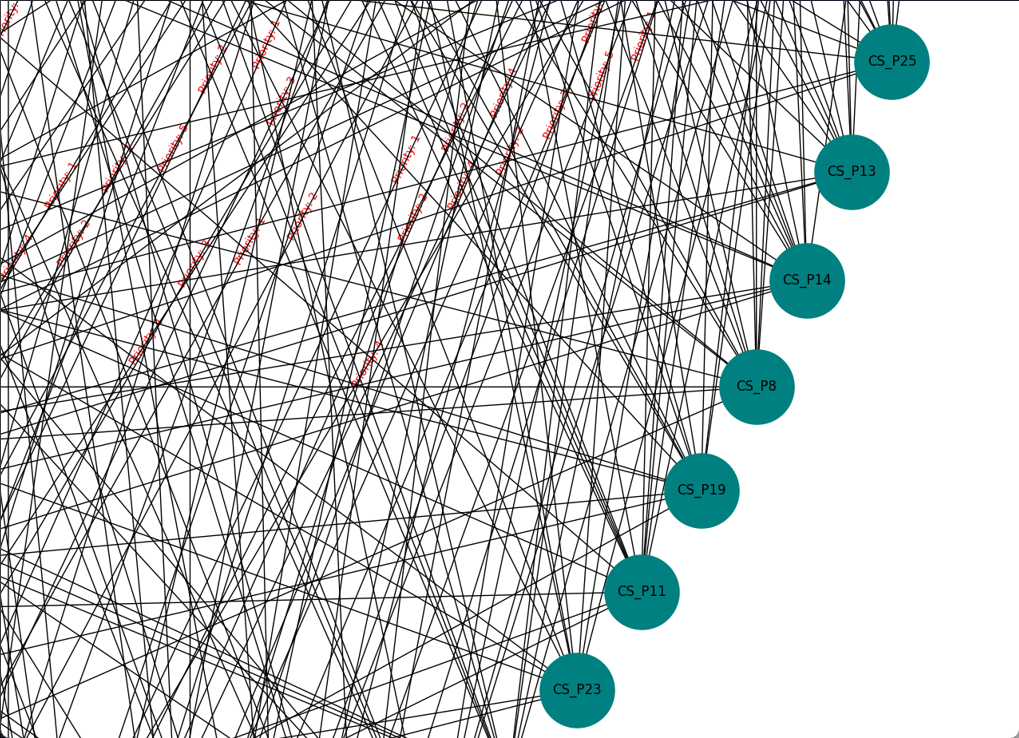
\includegraphics[scale =0.8]{Graph2}

The above graph was produced using networkx and Matplotlib.pyplot taking inputs from FileInput. Each node refers to the courses that are being allotted in the semester and the professors who are taking the courses. Every edge represents the connections that are made between the professor and the courses there in his or her priority list. Each edge also is marked with the priority at which the course is for the professor. \\ \\



\section{Code Implementation}

(i) All the input data were taken in as .csv files. The three most important files were ProffessorList, CourseList, and FileInput. ProfessorList includes the IDs of all the professors and maps them to the Professor Name and Professor Type. \\                                                        CourseList includes all the courses which are being offered in the semester. It contains the course code which maps it to the course name and course type.        \\   
FileInput is the data that contains all the course priorities of the professors. It contains the list of all the priority orders of the professors. Each professor has a choice to give a list of 16 courses in which they give their top priorities for each course type in a descending manner. The last column denotes the number of courses the professor can take in the semester. \\ 

%insert data file input
\graphicspath{ {./images/} }
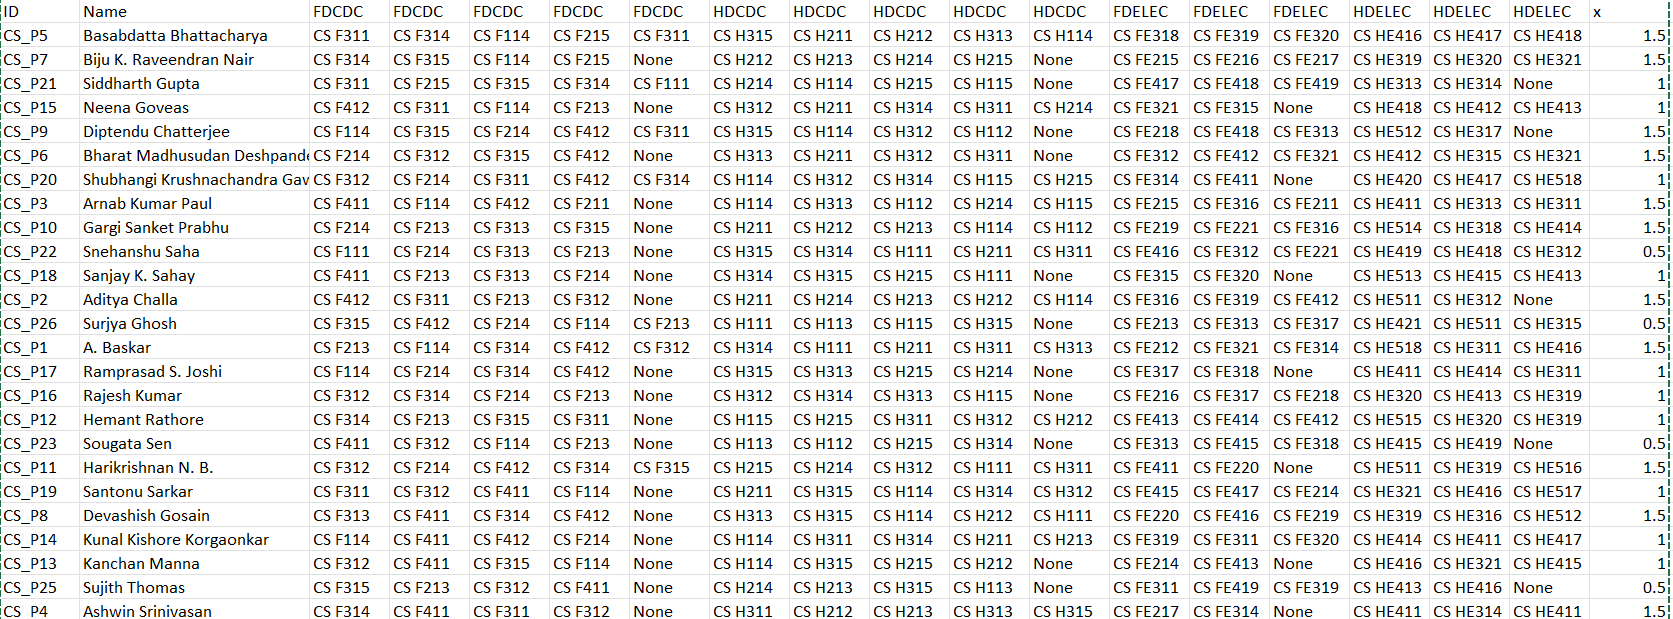
\includegraphics[width=\textwidth]{Data} \\ \\


(ii) The Professor.py file classifies and stores each professor’s priority. When a professor is assigned a course, the py file adds it to the data type “noOfCoursesTaken”. When a professor is assigned the maximum no. of courses they can take, they are made unavailable for the next course assignment. This ensures a professor does not take courses more than their type allows them to. \\ \\

%insert code snippet
\graphicspath{ {./images/} }
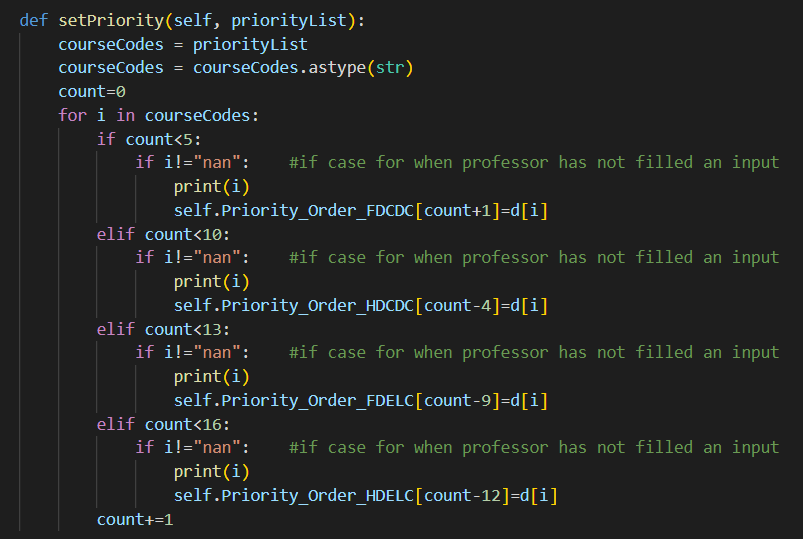
\includegraphics[width=8cm]{Professor.py1}
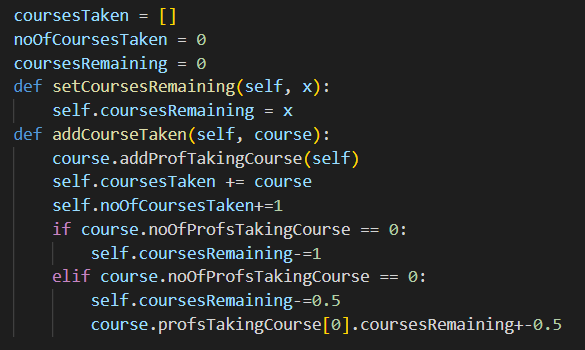
\includegraphics[width=10cm]{Professor.py2}\\
a)Course priorities being assigned for a professor   \hspace{1cm}       b)Professor availability for further course allotment \\ \\

\graphicspath{ {./images/} }
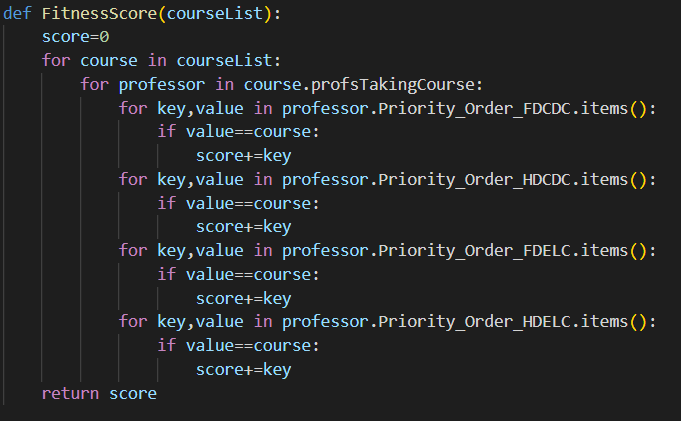
\includegraphics[width=\textwidth]{Fitness} \\ 
 \hspace{5cm} c) Fitness score is calculated based on course priorities.


\pagebreak


\section{Acknowledgement}
We would like to thank Sohil Khan for contributing to our code by providing different inputs on implementing the optimization problem solution in Python. We would also like to thank Professor Snehanshu Saha for allowing us to solve a real-life problem using the applications of graph theory.\\



\end{document}